% Innehållet i Vasungavisor 2010
%
% Kapitel "I Högan Nord"

\sclearpage
\songchapter{Ur Törstiga Strupar}
\begin{figure}[!b]
\begin{center}
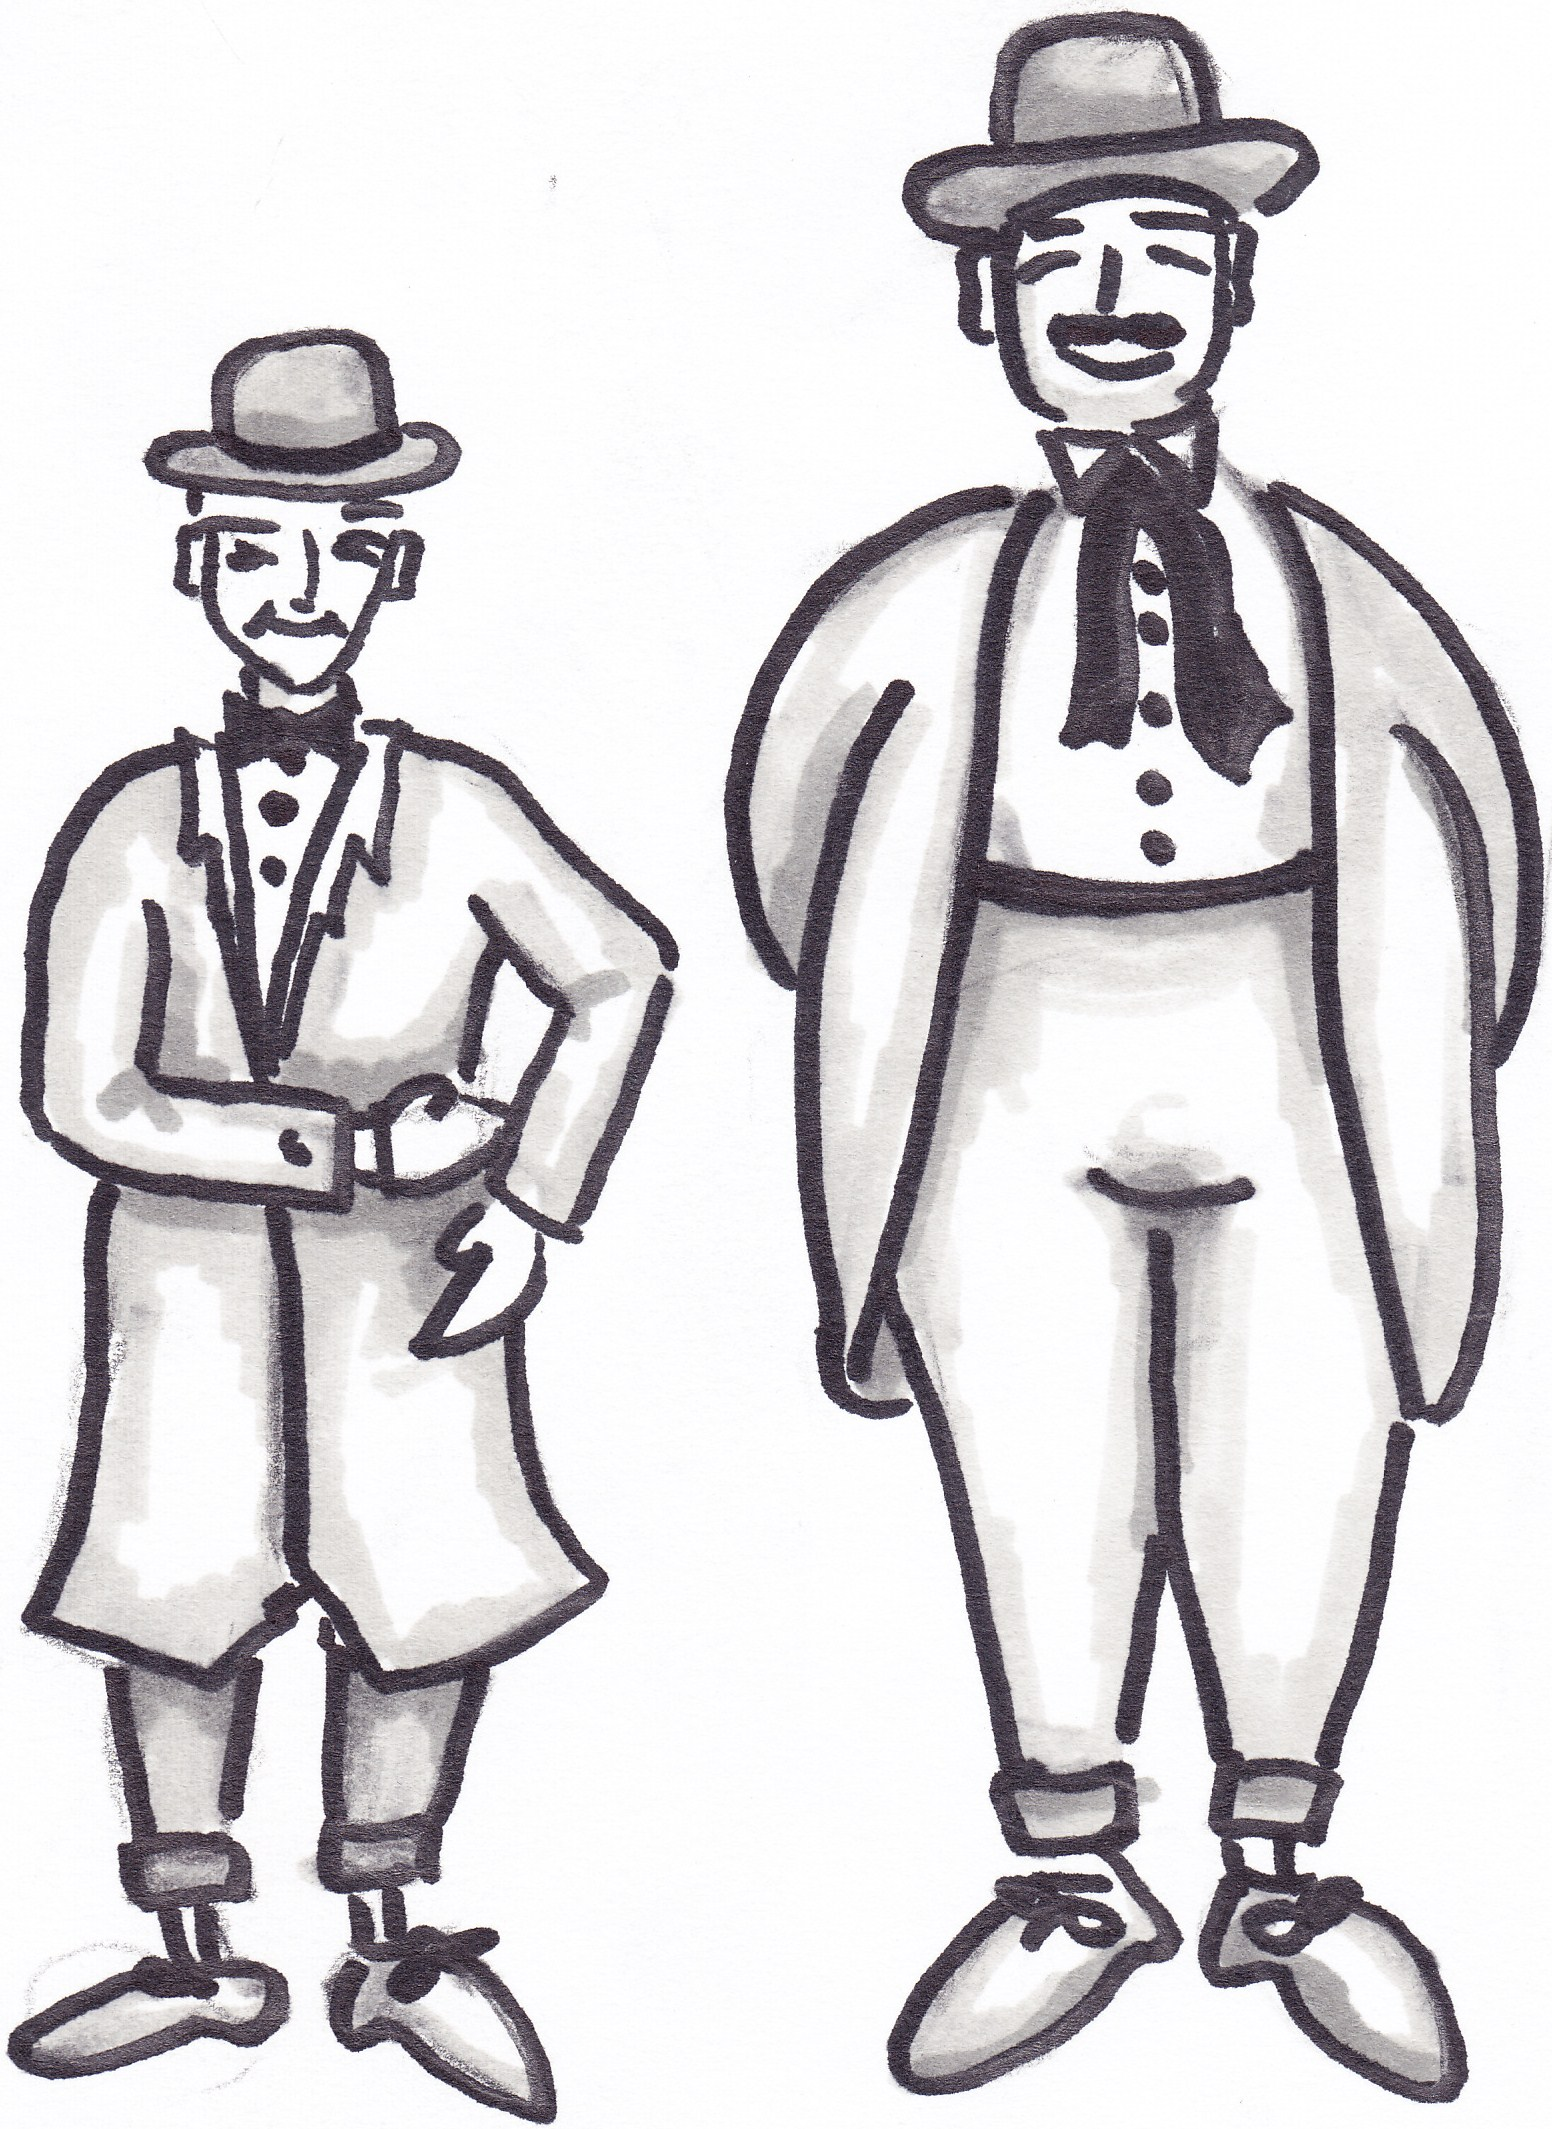
\includegraphics[width=5cm]{../bilder/helanochhalvan.jpg} 
\end{center}
\end{figure}
\sclearpage
\begin{intersong}

\textbf{SNAPSARNAS NAMN}

\begin{small}
Alltsedan den blida tid då vårt brännvin uppfanns, har umgänget med detsamma varit omgärdat av en stängeligen upprätthållen ritual. Vad vi vet därom förtäljer traditionen. Brännvinet inmundigades i bestämda kvantiteter benämnda "Snapsen" eller "Supen". Enär dessa av goda skäl inte kunde tillåtas intagas godtyckligen, fick de snart alltefter sina rituella ordningsnummer specifika namn, av vilka vi idag känna tretton. Dessa är Helan, Halfvan, Tersen, Quarten, Quinten, Rifvan, Rafflan, Rännan, Smuttan, Smuttans unge, Femton droppar, Lilla Manasse och Lilla Manasses broder. Detta kulturarv bjuder oss att följa denna ritual och inte tillåta stundens nycker nagga dryckesdisciplinen i kanten. Vad skulle våra dryckesfäder känna i sina hjärtan om de från sina molnkanter nedblickade på en snapsritual innehållande "Langbeinakrank" istället för Rifvan och "Tjorven" eller, hemska tanke "Sjunkbomben" istället för den ärevördiga Lilla Manassen? Ruelse och vemod! Sentida studenter plägnar dock att utöver de traditionella alltefter tillfället tillägga snapsarna Kreaturets återuppståndelse och Inspektors klagan. Detta kunde emellertid klandras med avseende på måttlighet i denna värld befolkad av ett i fysisk måtto något förvekligat släkte, men som bekant tillhör inte omåttlighet dödssynderna, ej heller är måttlighet den högsta av dygder. Dock torde detta gruvligen utökade antalet snapsar anses vara ett förvekligat släkte tillfyllest. Efterföljande samling gör inte anspråk på uttömlighet ifråga om de olika smakriktningarna inom supvisornas genre, från tradition till vomeringsromantik, men likförbannat bör de uppstämmas med samma kraft som fordom innan snapsen under andaktsfull tystnad intagas. I kvistiga fall angående melodi eller dryckesdisciplin torde man vända sig till någon äldre vasung, lämpligen sångledaren (vasungen med sångvärjan; akta dig för den, du).
\end{small}

\end{intersong}


\sclearpage
\beginsong{Helan}					
	
\beginverse*
Helan går, 
sjung hoppfaderallallallallej
helan går, 
sjung hoppfaderallallej!
Och den som inte helan tar, 
han ej heller halvan får. 
Helan går, 
sjung hoppfaderallallej!			
\endverse									
\endsong							

\beginsong{Halvan}[
		sr={Så väva vi vadmal},
		index={Så väva vi vallman}]
					
\beginverse*						
Så väva vi vallman,
så taga vi halvan.
Väva vallman och taga halvan
och låta suparna gå, gå.
\endverse		
\endsong
\beginsong{Tersen}[
		sr={},
		index={Fjärran han dröjer}]

\beginverse*						
Fjärran han dröjer ur törstiga strupar, 
redan vi tagit två modiga supar. 
Ack, lilla tersen, ack, lilla hjärtevännen, 
kommer du ej snart? Jo, jag kommer STRAX!
\endverse		
\endsong
\sclearpage
\beginsong{Kvarten}[
		sr={Å jänta å ja'},
		index={Å tersen var bra}]

\beginverse*						
Å tersen var bra, å tersen var bra
och nu tar vi lilla kvarten hurra!
Å tersen var bra, å tersen var bra
och nu tar vi lilla kvarten.
När man den lilla tersen har fått,
smakar den lilla kvarten så gott,
och den smaken har vi aldrig försmått.
Hipp, hipp hurra för Småttin!
\endverse		
\endsong
\beginsong{Kvinten}					
	
\beginverse*
GE MIG TEXT!!!
\endverse									
\endsong							

\sclearpage
\input{Halvankaren.tex}
\input{DenSallskapssjukaHalvan.tex}
\sclearpage
\input{DetSattEnMas.tex}
\begin{figure}[!b]
\begin{center}
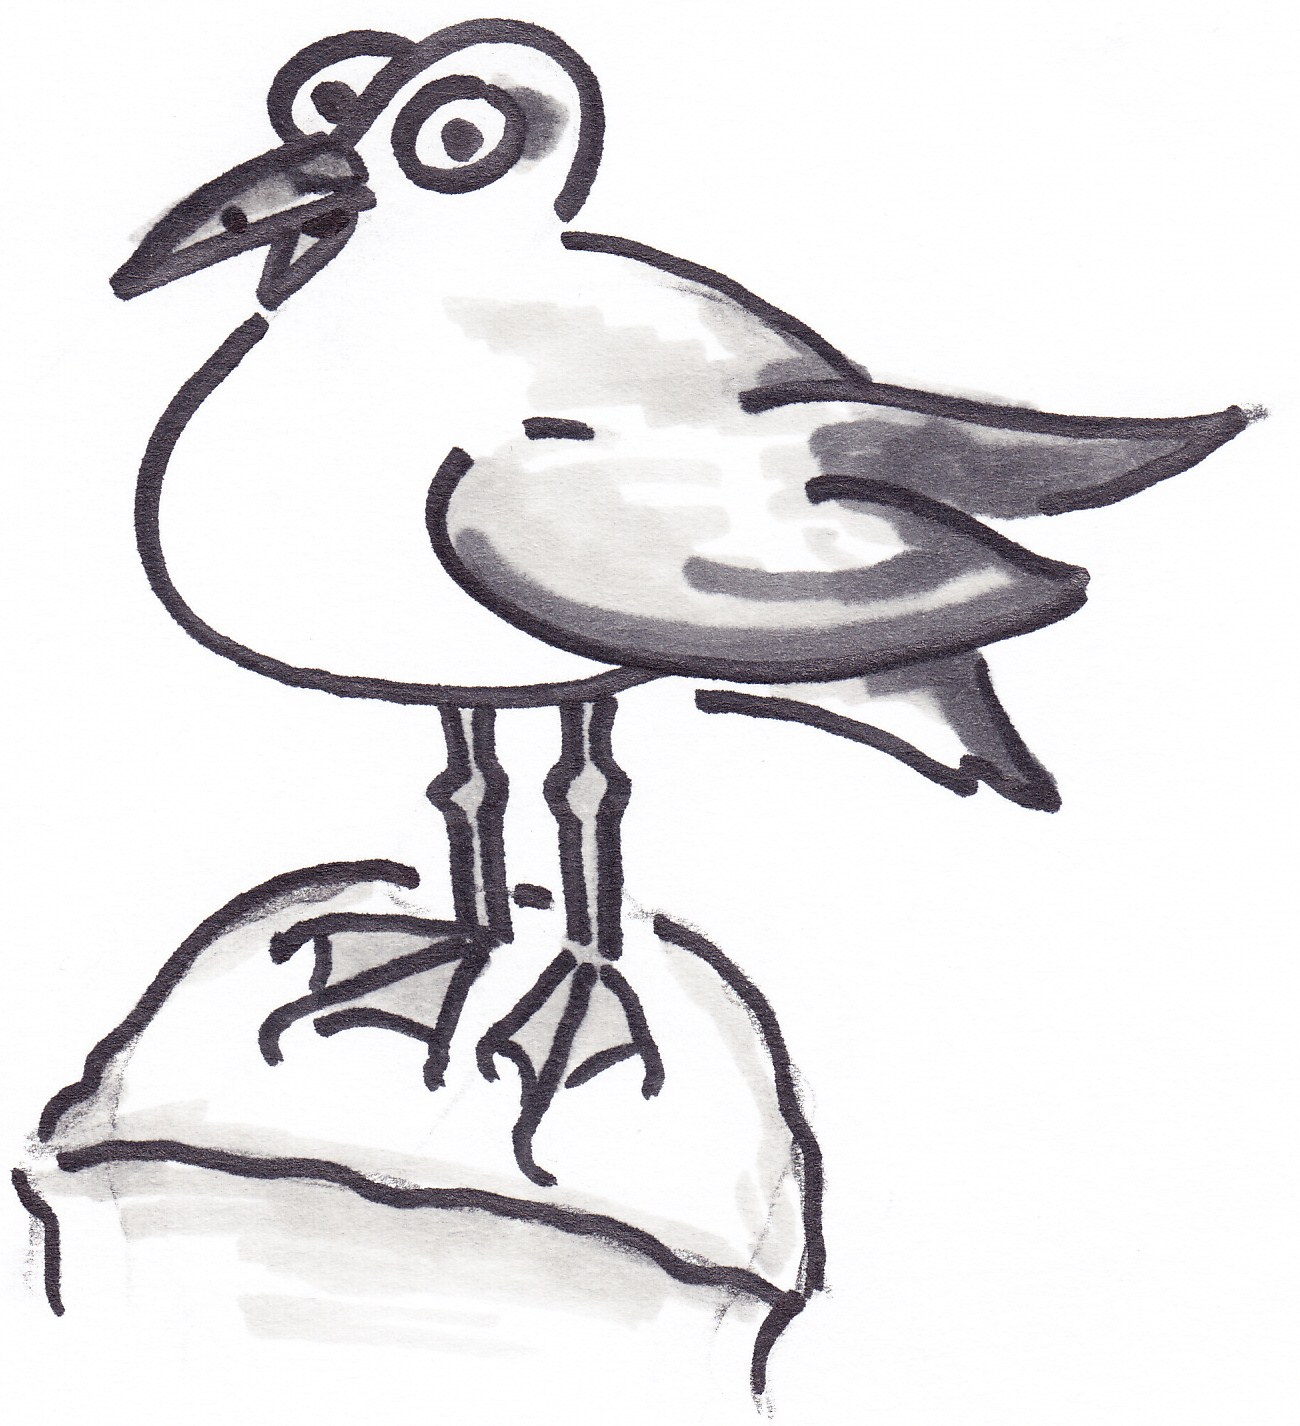
\includegraphics[width=25mm]{../bilder/mas.jpg} 
\end{center}
\end{figure}
\sclearpage
\beginsong{Gå på fest}[ 							
	sr={Du ska få min gamla cykel},					
	index={När som livet kännes},
	index={Är du vissen}]		
	
\beginverse*						
När som livet kännes mörkt och grått och trist,
GÅ PÅ FEST
När humöret allt emedan du mist,
GÅ PÅ FEST
När du tror att allting grånar, 
ska du se att himlen blånar, 
sommarns blommor dig förvånar, 
GÅ PÅ FEST!
\endverse						

\beginverse				
Är du vissen, klen och trött och matt och svag, 
GÅ PÅ FEST
Skulle hjärtat bara slå vartannat slag, 
GÅ PÅ FEST
Strunt i doktorn och recepter, 
medicin och farmacepter, 
sluta upp och känna efter, 
GÅ PÅ FEST!
\endverse				
\endsong		

\sclearpage
\beginsong{Härjarvisan}[ 	
    by={Hasse Alfredsson},						
	sr={Gärdebylåten},					
	index={Nu ska vi ut och härja}]		

\beginverse*
Liksom våra fäder vikingarna i Norden,
drar vi landet runt och super oss under borden.
Brännvinet har blitt ett elexir 
för kropp såväl som själ.
Känner du dig liten och ynklig på jorden,
växer du med supen och blir stor uti orden.
Slår dig för ditt håriga bröst,
och blir en man från hår till häl.
\endverse

\beginchorus				
Ja, nu skall vi ut och härja,
supa och slåss och svärja,
bränna röda stugor, slå små barn
 och säga fula ord!
Med blod skall vi stäppen färga.
Nu änteligen lär jag
kunna dra nån riktig nytta av
min Hermodskurs i mord! 
\endchorus	

\beginverse					
Hurra, nu skall man äntligen få röra på benen,
hela stammen jublar och det spritter i grenen.
Tänk att än en gång få spränga fram
 på Brunte i galopp!
Din doft, o kära Brunte är trots brist i hygienen,
för en vild mongol minst lika ljuv som syrenen.
Tänk att på din rygg få rida runt
 i stan och spela topp. 
\endverse						

\beginchorus				
Ja, nu skall vi ut och härja ...
\endchorus	

\beginverse
Ja, mordbänder är klämmiga, ta fram fotogenen!
Och eftersläckningen tillhör just de fenomenen
inom brandmansyrket, som jag tycker 
det är nån nytta med.
Jag målar för mitt inre upp den härliga scenen: 
blodrött mitt i brandgult. Ej ens prins Eugen en
lika mustig vy kunnat måla, 
ens om han målade med sked. 
\endverse	

\beginchorus	
Ja, nu skall vi ut och härja ... 
\endchorus	

\vspace{5mm}
\endsong		

\input{FordomOdladeMan.tex}
\sclearpage
\beginsong{Heppeneppetepp}[ 						
	index={Till Stockholm for}]		
	
\beginverse*						
Till Stockholm for Heppeneppetepp, 
till Stockholm for jag.
Till Stockholm for Heppeneppetepp,
till Stockholm for jag.
\endverse	
\beginchorus
:,: Till Stockholm for Amalia
som bad oss supa bra, 
och till Stockholm for alla raska gossar
som i laget där var. :,:
\endchorus		

\beginverse				
Och supen tog Heppeneppetepp
och supen tog jag.
Och supen tog Heppeneppetepp
och supen tog jag.
\endverse	
\beginchorus
:,: Och supen tog Amalia... :,:
\endchorus	

\beginverse
I finkan kom Heppeneppetepp
i finkan kom jag. 
I finkan kom Heppeneppetepp
i finkan kom jag.
\endverse	
\beginchorus
:,: I finkan kom Amalia... :,:
\endchorus

\beginverse
Men frikänd blev Heppeneppetepp
och frikänd blev jag. 
Men frikänd blev Heppeneppetepp
och frikänd blev jag. 
\endverse	
\beginchorus
:,: Och frikänd blev Amalia... :,:
\endchorus	
\endsong		

\sclearpage


\beginsong{Hur länge skall på bordet}[
	index={Det ärvda vikingsinne}]		
	
\beginverse*						
Hur länge skall på bordet
den lilla halvan stå?
Skall snart ej höras orden:
Låt halvan gå, låt gå!
Det ärvda vikingasinne till supen trår igen 
Och helans trogna minne i halvan går igen. 
\endverse									
\vspace{5mm}
\endsong		

\beginsong{Det perfekta glaset}[
	by={Nicklas Forss},
	sr={Sommardag i Kangasala},
	index={Jag lyfte den lilla supen}]
	
\beginverse*						
Jag lyfte den lilla supen
och hällde den i min hals.
Det kittla så härligt i strupen,
men kvar fanns sen inget alls.
Jag titta på glaset och drömde
att det hade sådan funktion:
:,: hur mycket man än ur det tömde,
där alltid fanns kvar en portion. :,:
\endverse						
\endsong		

\sclearpage
\beginsong{Kassen full}[				
	sr={Vinden drar}]		
	
\beginverse*						
Kassen full
förbi vår tull
hämtar jag hem med mig.
Jag hämtar brännvin, genever och gin
och allt så dricker jag själv. 
\endverse		
		
\vspace{5mm}
\endsong		

\input{Infinitesimaldifferensen.tex}
\sclearpage
% Exempel på färdig-formaterad sång till VN:s
% sångbok 2010.

% Denna fil kan användas som sådan, bara verserna,
% namnen och annan rådata behöver bytas ur fälten.
% Tecknet "%" markerar en kommentar som helt och 
% hållet ignoreras av programmet som läser filen.

% Spara den färdiga filen som 
% 'SangnamnUtanMellanslagEllerSkander.tex'
% t.ex. blir "Vid En Källa" till 
% 'VidEnKalla.tex'
% Varje sång blir en egen fil.

\beginsong{Jag har aldrig vart på snusen}[ 	% Börja sången här
	by={},	% Författare
	sr={O hur saligt att få vandra}]		% Alternativa
			% sångnamn
	
\beginverse*		% Börja vers
Jag har aldrig vatt på snusen,
aldrig rökat en cigarr - halleluja!
Mina dygder äro tusen,
inga syndiga laster jag har.
\endverse
\beginverse*
Jag har aldrig sett nå't naket,
inte ens ett litet nyfött barn.
Mina blickar går mot taket,
därmed undgår jag frestarens garn.
\endverse			% Sluta vers

\beginchorus
Halleluja, halleluja, 
halleluja, halleluja
halleluja, halleluja,
Hallelujaaa-aaa-a!
\endchorus

\beginverse*		% Börja vers
Bachus spelar på gitarren,
Satan spelar på sitt handklaver.
Alla djävlar dansar tango,
säg vad kan man väl önska sig mer?
\endverse
\beginverse*
Jo, att alla bäckar vore brännvin,
stadsparksdammen full av bayerskt öl,
konjak i varenda rännsten
och punsch i varendaste pöl.
\endverse			% Sluta vers

\beginchorus
Halleluja, halleluja...
\endchorus
\endsong			% Sluta sång

\sclearpage
\input{Kosmonauten.tex}
\begin{figure}[!t]
\begin{center}
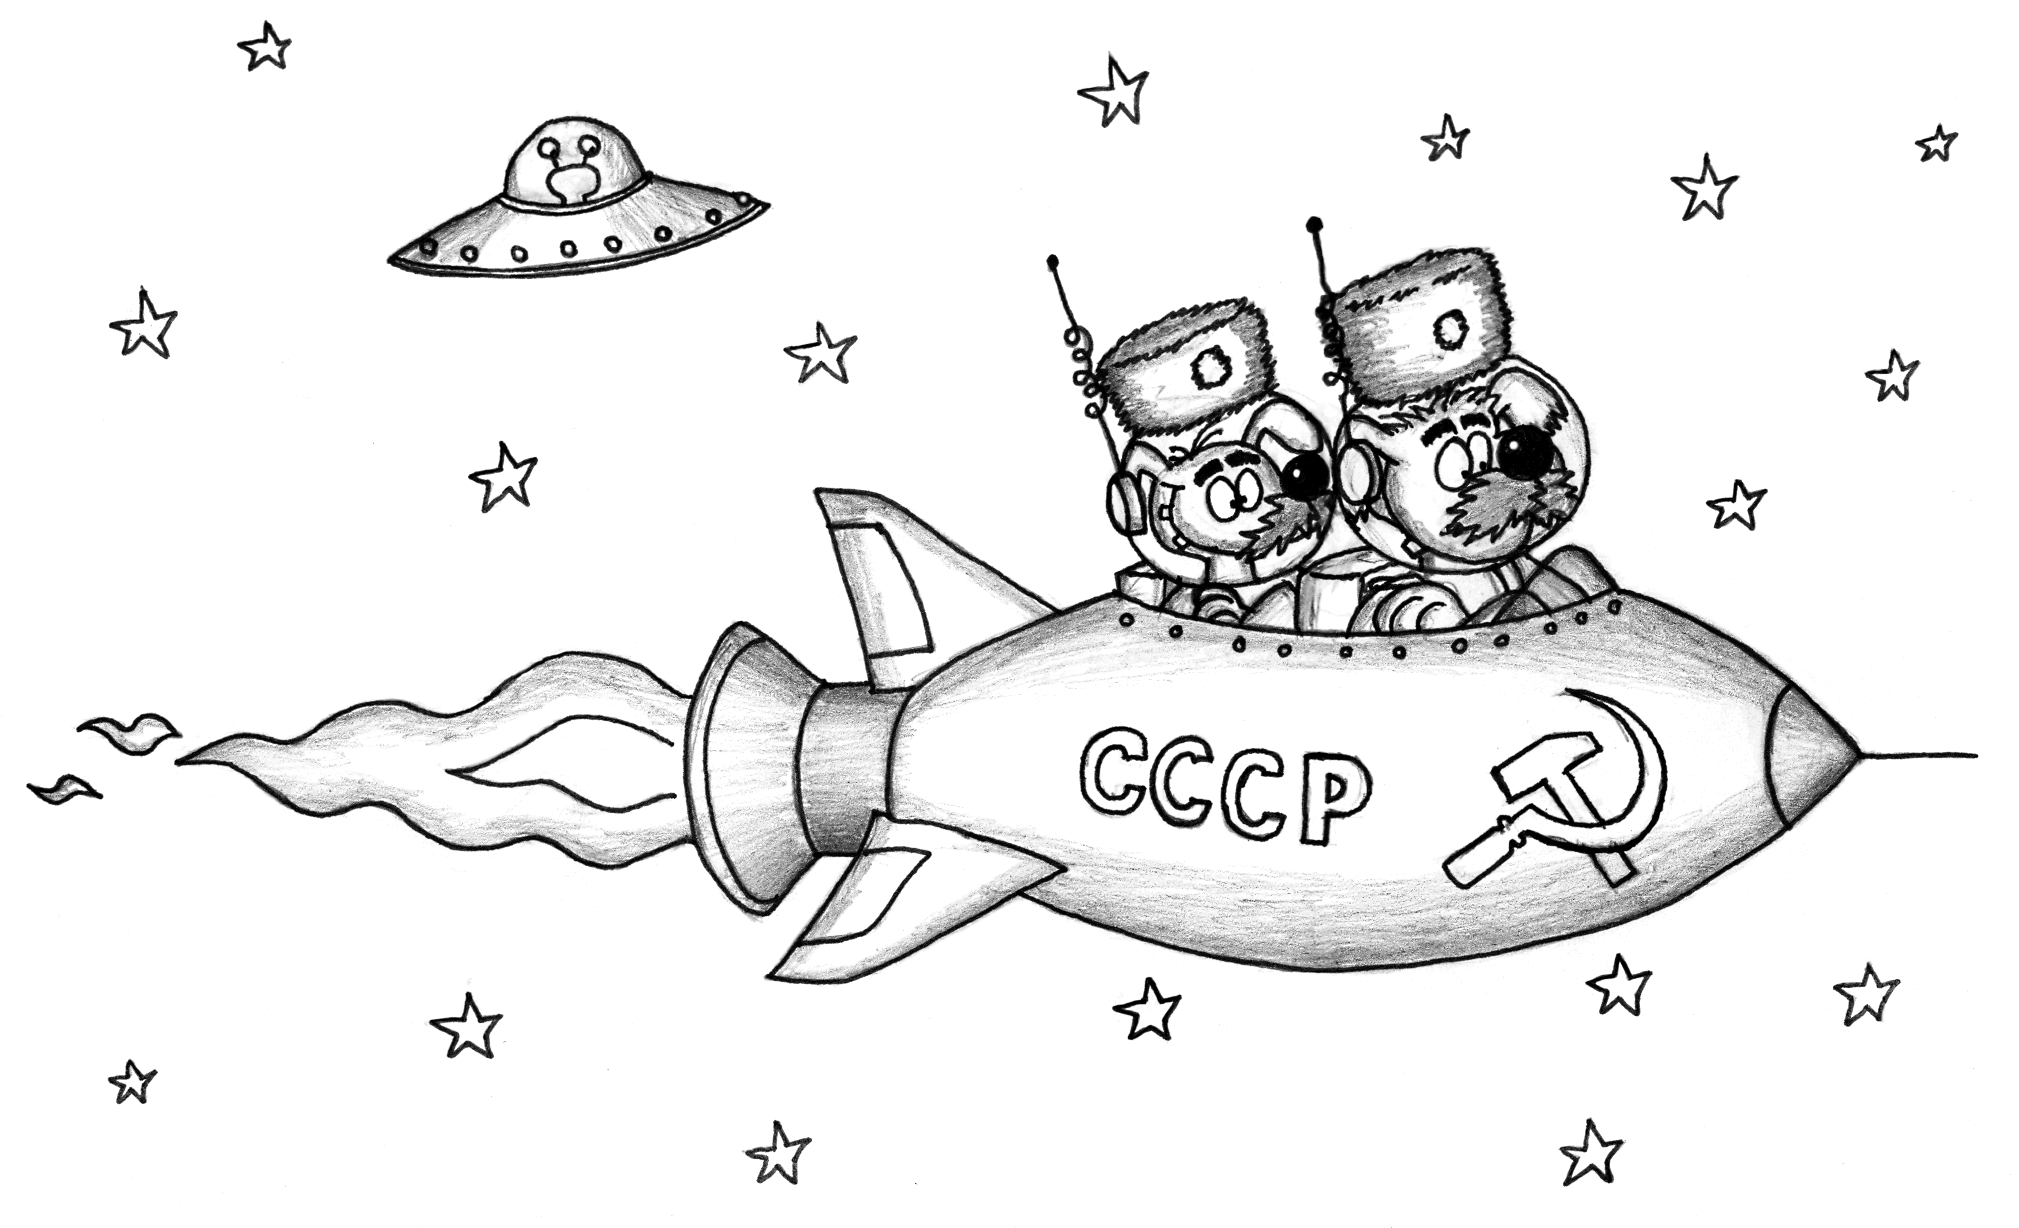
\includegraphics[width=6cm]{../bilder/kosmonauten.png} 
\end{center}
\end{figure}
\vspace{25mm}
\beginsong{Mitt lilla lån}[ 						
	sr={Hej tomtegubbar}]	
	
\beginverse*						
:,: Mitt lilla lån det räcker inte, det går till öl och till brännvin! :,:
Till öl och brännvin går det åt, 
och så till pojkar/flickor/pepparkaksindivider emellanåt.
Mitt lilla lån det räcker inte, 
det går till öl och till brännvin
\endverse				
\endsong		

\sclearpage
\beginsong{Livet är härligt}[ 							
	sr={Pråmdragarna på Volga},
	index={Ta dig en vodka}]		
	
\beginverse*						
Livet är härligt,
tavaritj, vårt liv är härligt!
Vi alla våra små bekymmer glömmer, 
när vi har fått en tår på tand; en skål!,
\endverse						

\beginverse				
Ta dig en vodka, 
tavaritj, en liten vodka! 
Glasen i botten vi tillsammans tömmer,
det kommer mera efter hand; en skål!
\endverse

\textnote{Sången sponsoreras av Vasa nations inspektor 2015- Ilse Julkunen.}
\endsong		

\begin{figure}[!b]
\begin{center}
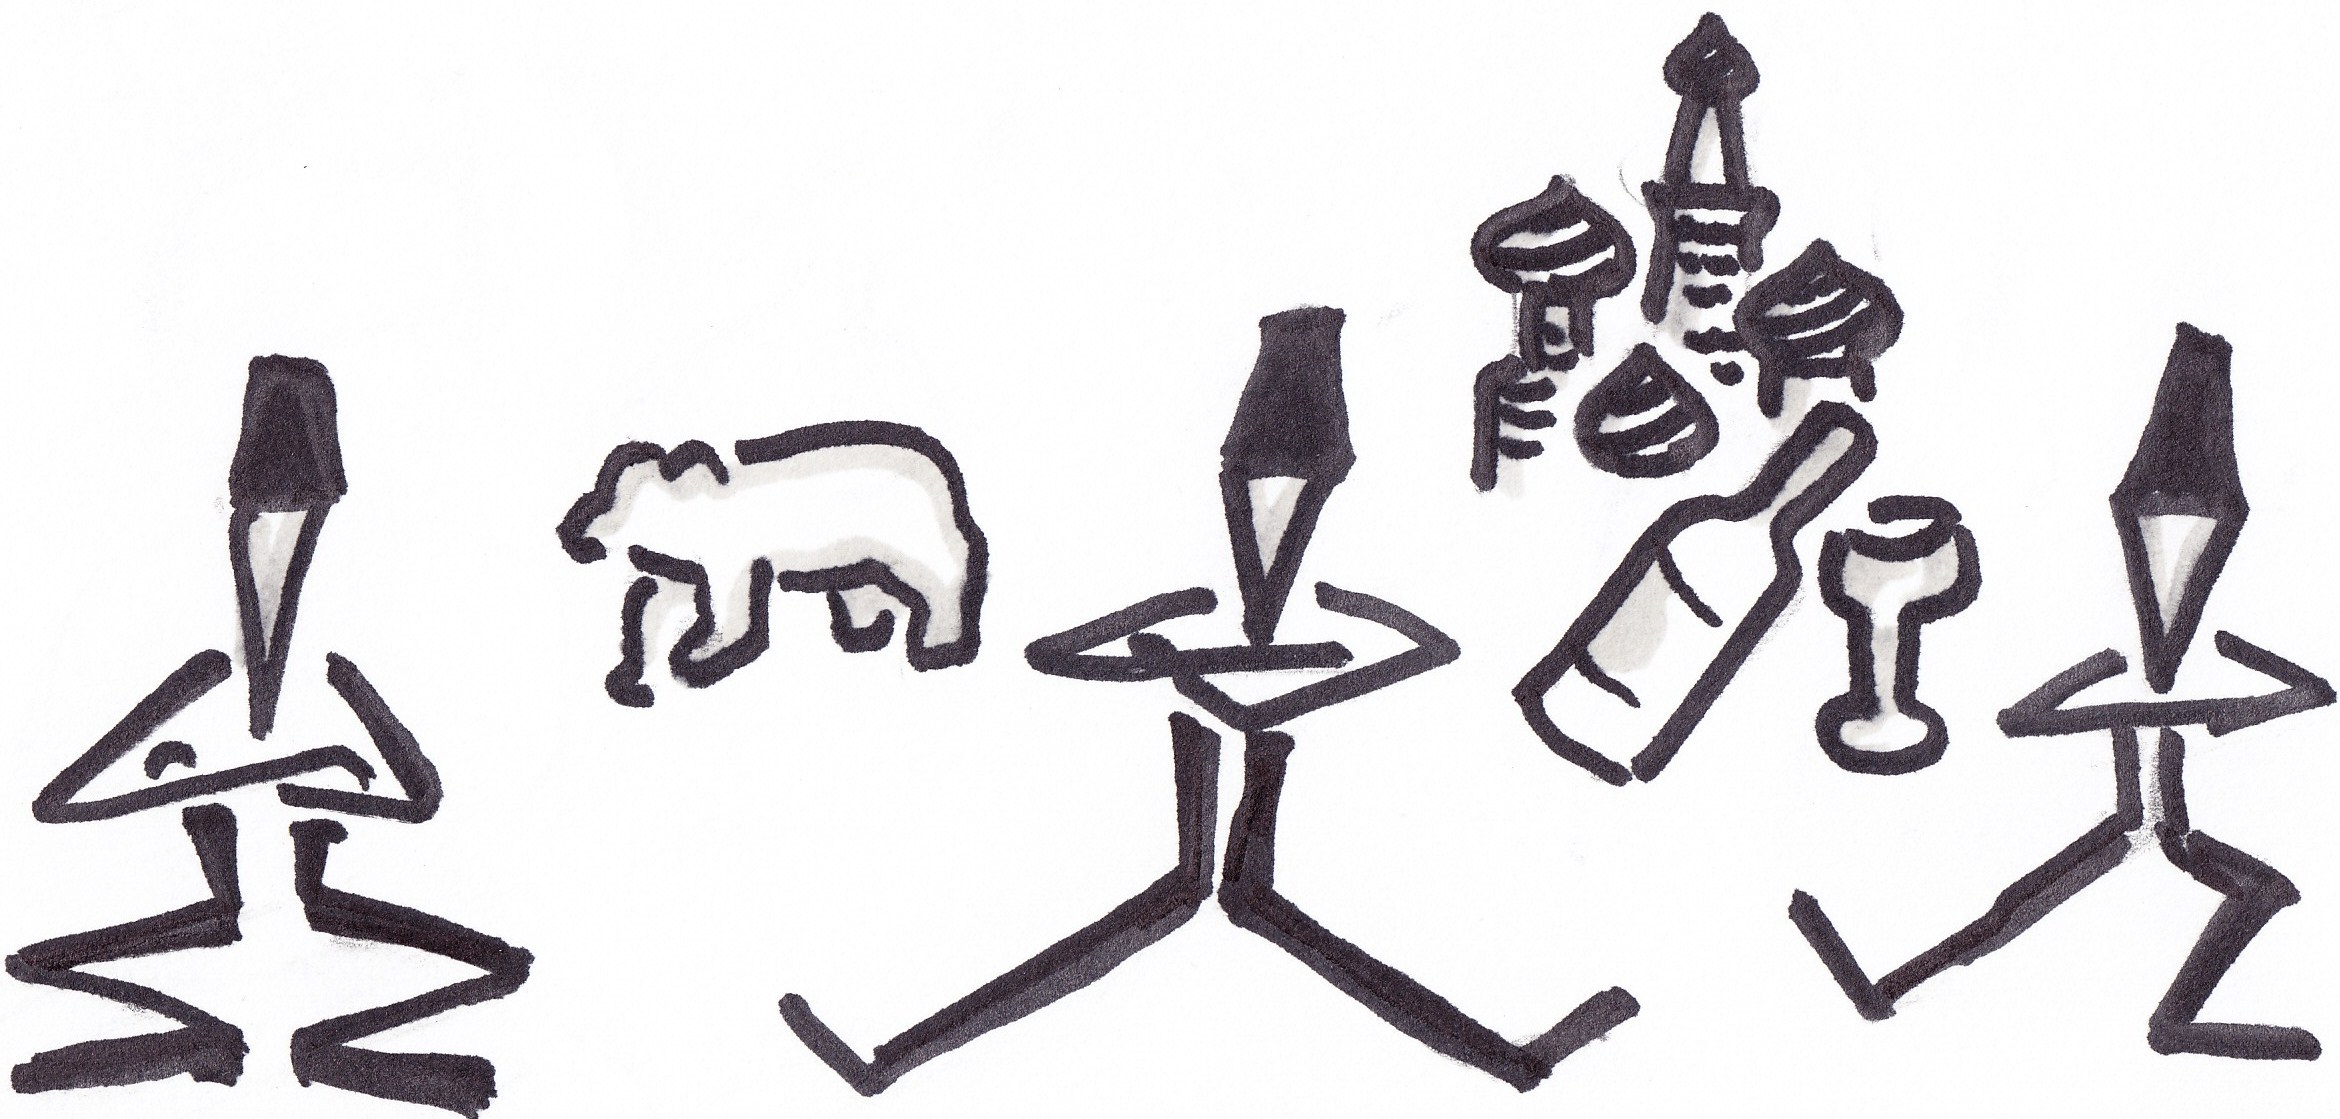
\includegraphics[width=6cm]{../bilder/livet_ar_harligt.jpg} 
\end{center}
\end{figure}
\clearpage
\sclearpage
\beginsong{Mera brännvin}[ 						
	sr={Internationalen},					
	index={Internationalen}]		
	
\beginverse*						
Mera brännvin i glasen,
mera glas på vårt bord,
mera bord på kalasen,
mer kalas på vår jord.
\endverse						

\beginverse				
Mera jordar kring månen,
mera månar kring Mars,
mera marscher till Skåne,
mera Skåne - bevars!
\endverse			

\beginverse*						
Lisää viinaa mun lasiin,
lisää laseja pöydälle,
lisää pöytiä näihin juhliin,
lisää juhlia kansalle.
\endverse					

\beginverse				
Lisää kansaa Suomeen,
lisää Suomea päälle maan,
lisää maata Suur-Suomelle,
marssitaan, marssitaan, Karjalaan, Karjalaan! 
\endverse					

\vspace{1cm}	
\endsong		

\beginsong{Om cykling}[ 		
	by={Povel Ramel},					
	sr={Så väva vi vallman},					
	index={Man cyklar för litet}]		
	
\beginverse*						
Man cyklar för litet, 
Man röker för mycket.
Och man är fasen så liberal 
när det gäller maten och spriten. 
Man borde slutat för länge sedan
men denna sup är för liten. 
\endverse										

\beginverse*						
Vad tjänar att hyckla? 
Tids nog får man cykla! 
\endverse										

\endsong		

\sclearpage
\beginsong{Minnet}[ 		
	by={T. Perret},					
	sr={Memories}]		
	
\beginverse*						
Minne! 
Jag har tappat mitt minne! 
Är jag svensk eller finne? 
Kommer inte ihåg.
Inne!
Är jag ut eller inne? 
Jag har luckor i minne, 
sån' där små alkohål. 
Men besinn' er, 
man tätar med det brännvin man får, 
när som minnet och helan går. 
\endverse						

\beginverse				
 Minne? Muisti hävis, mutt' minne?
Juhlista selvisimme
- muistikatkoja on.
Minne, lähtisin vaikka minne,
kunhan selvittäisimme
mitä tapahtunut on.
Mutta tiedän
mä keinon mikä auttaapi tuo:
Ota ryyppy, ja muistis juo!\endverse				
\endsong		

\sclearpage
\input{Presidentvisan.tex}
\begin{figure}[!b]
\begin{center}
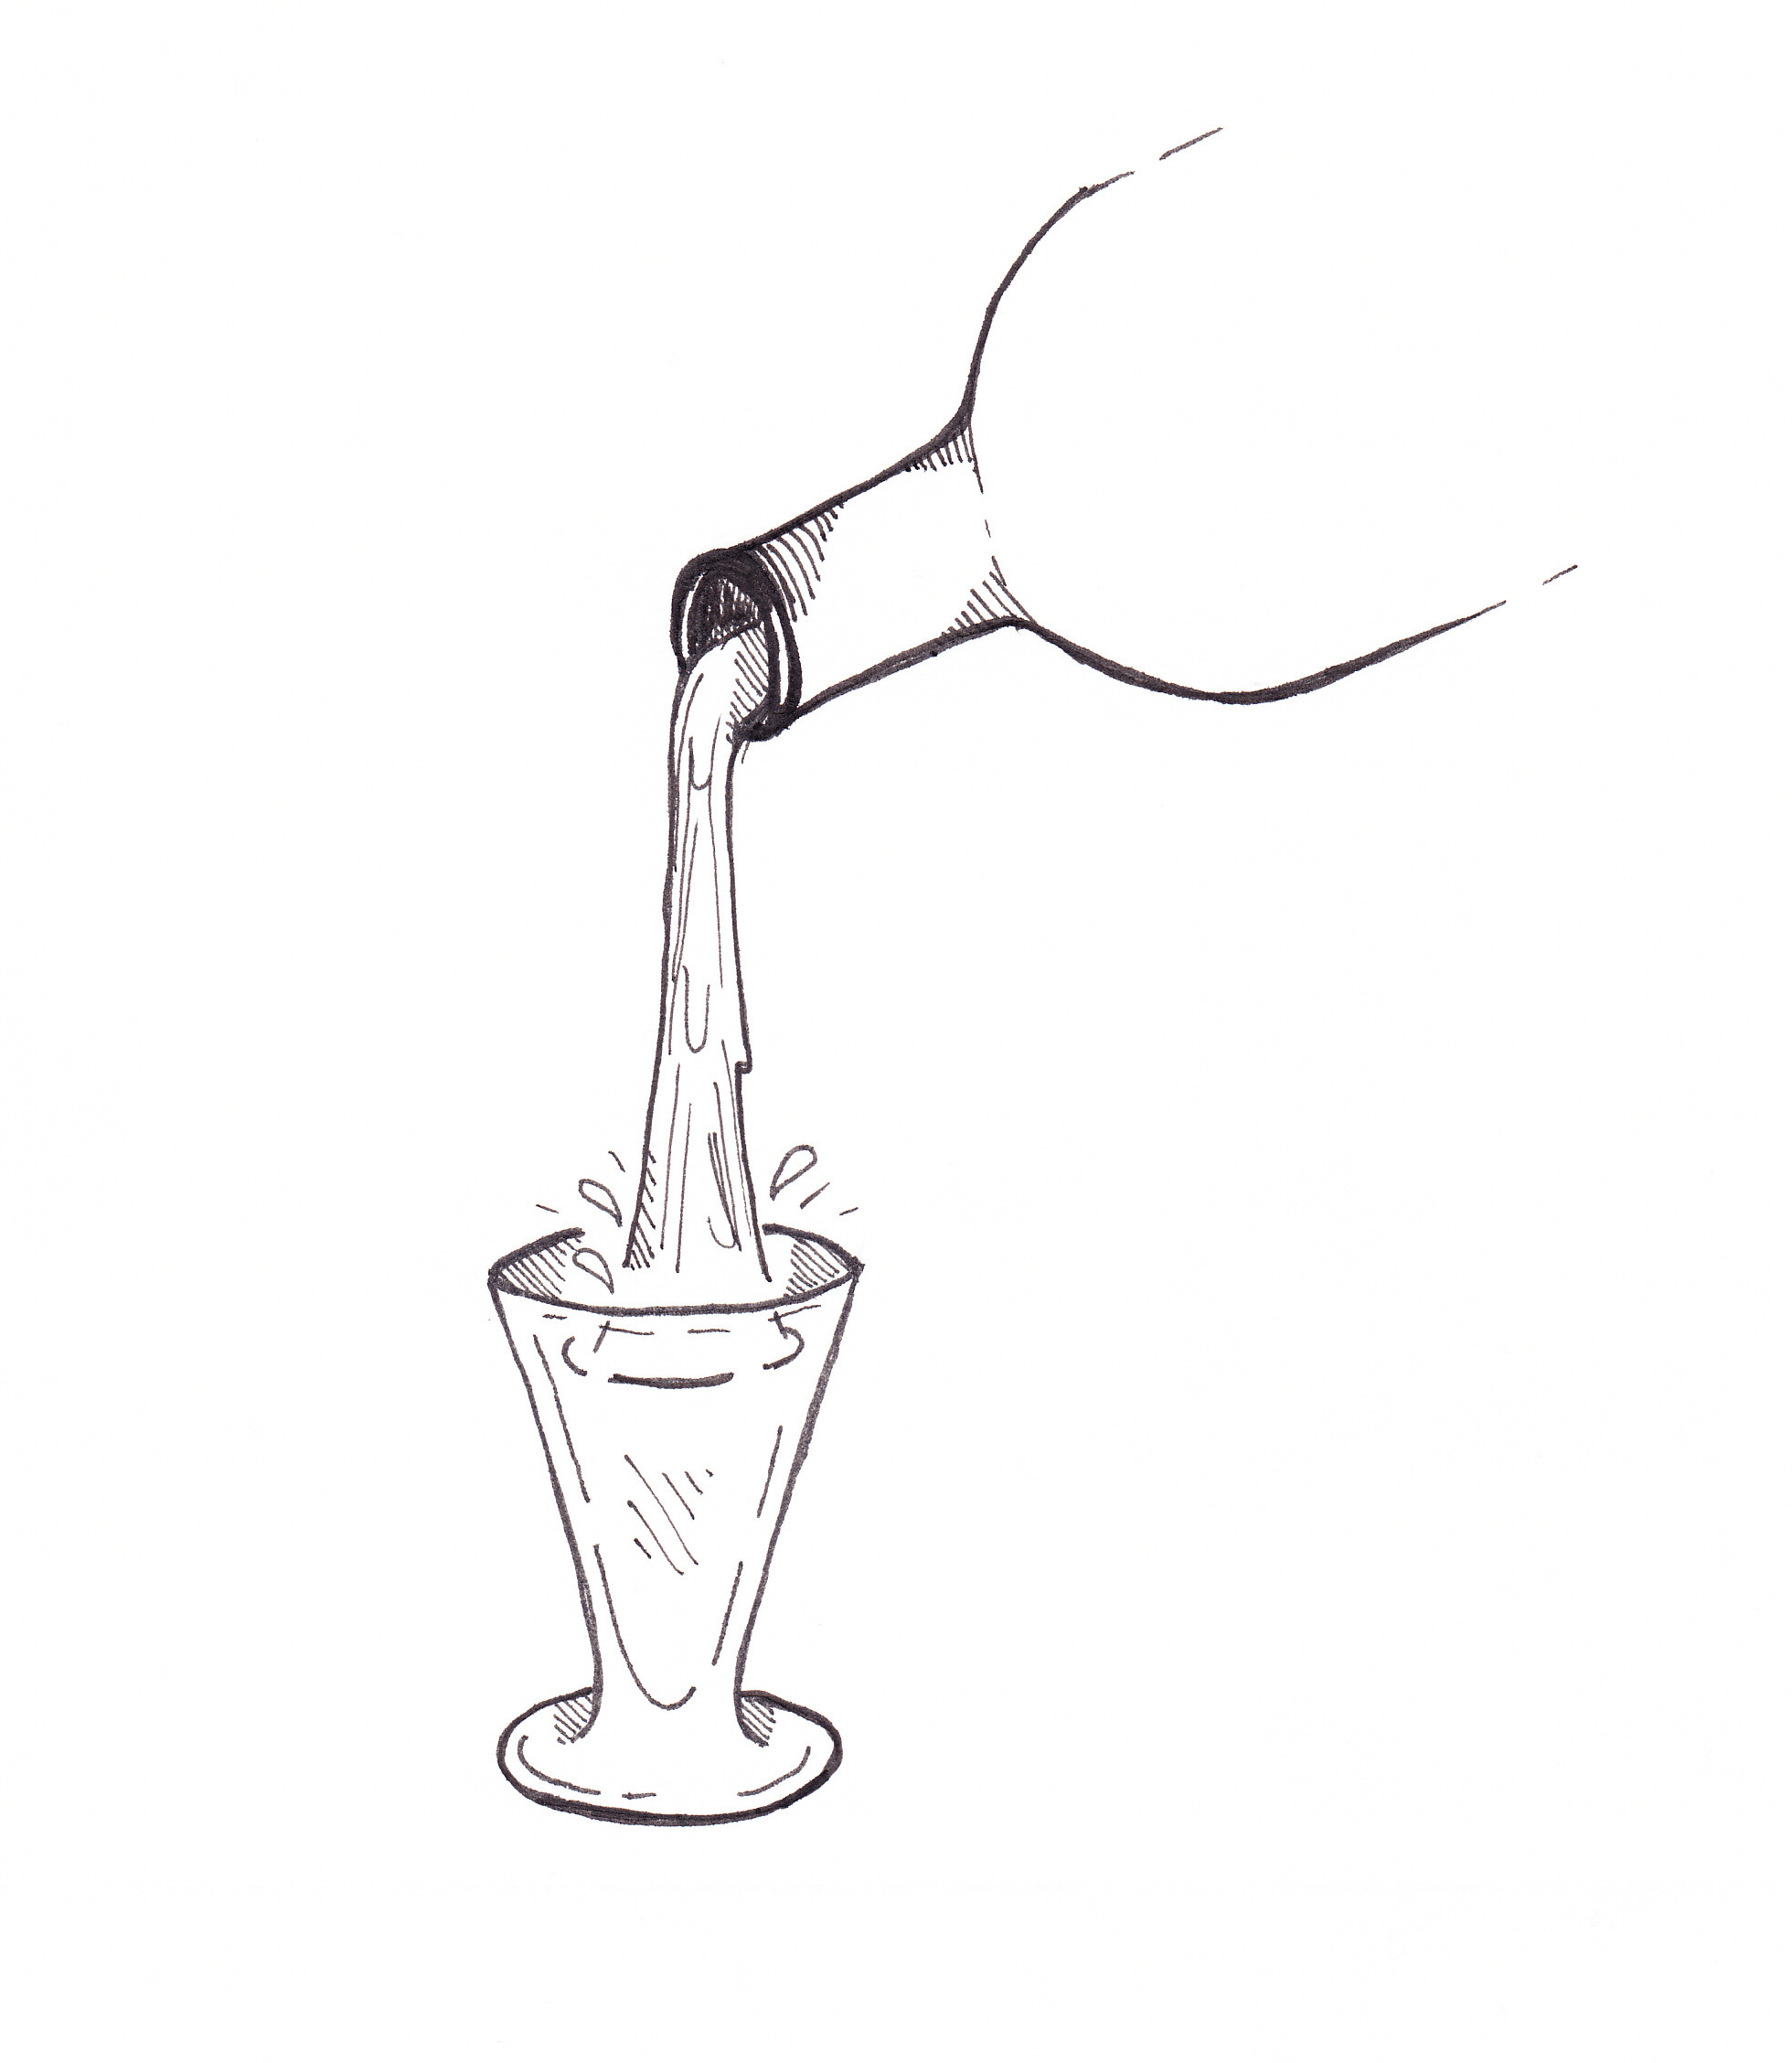
\includegraphics[width=30mm]{../bilder/hallandeflaska.jpg} 
\end{center}
\end{figure}
\sclearpage
\input{Rattataa.tex}
\sclearpage
\input{RenHelanSlunkitNer.tex}
\sclearpage
\beginsong{Brännvin, vatten}[ 	
	by={Atte och Jocke Boström},					
	index={Viinaa, vettä}]		
	
\beginverse*						
Brännvin, vatten,
 smakar skit som katten. 
Brännvin, helt rått,
 :,: smakar jävligt gott! :,:
\endverse
						
\beginverse				
Viinaa, vettä 
- mitä perkelettä? 
Viinaa raakaa 
:,: napaan kaatakaa! :,:
\endverse			

\vspace{1cm}	
\endsong		

\begin{figure}[!b]
\begin{center}
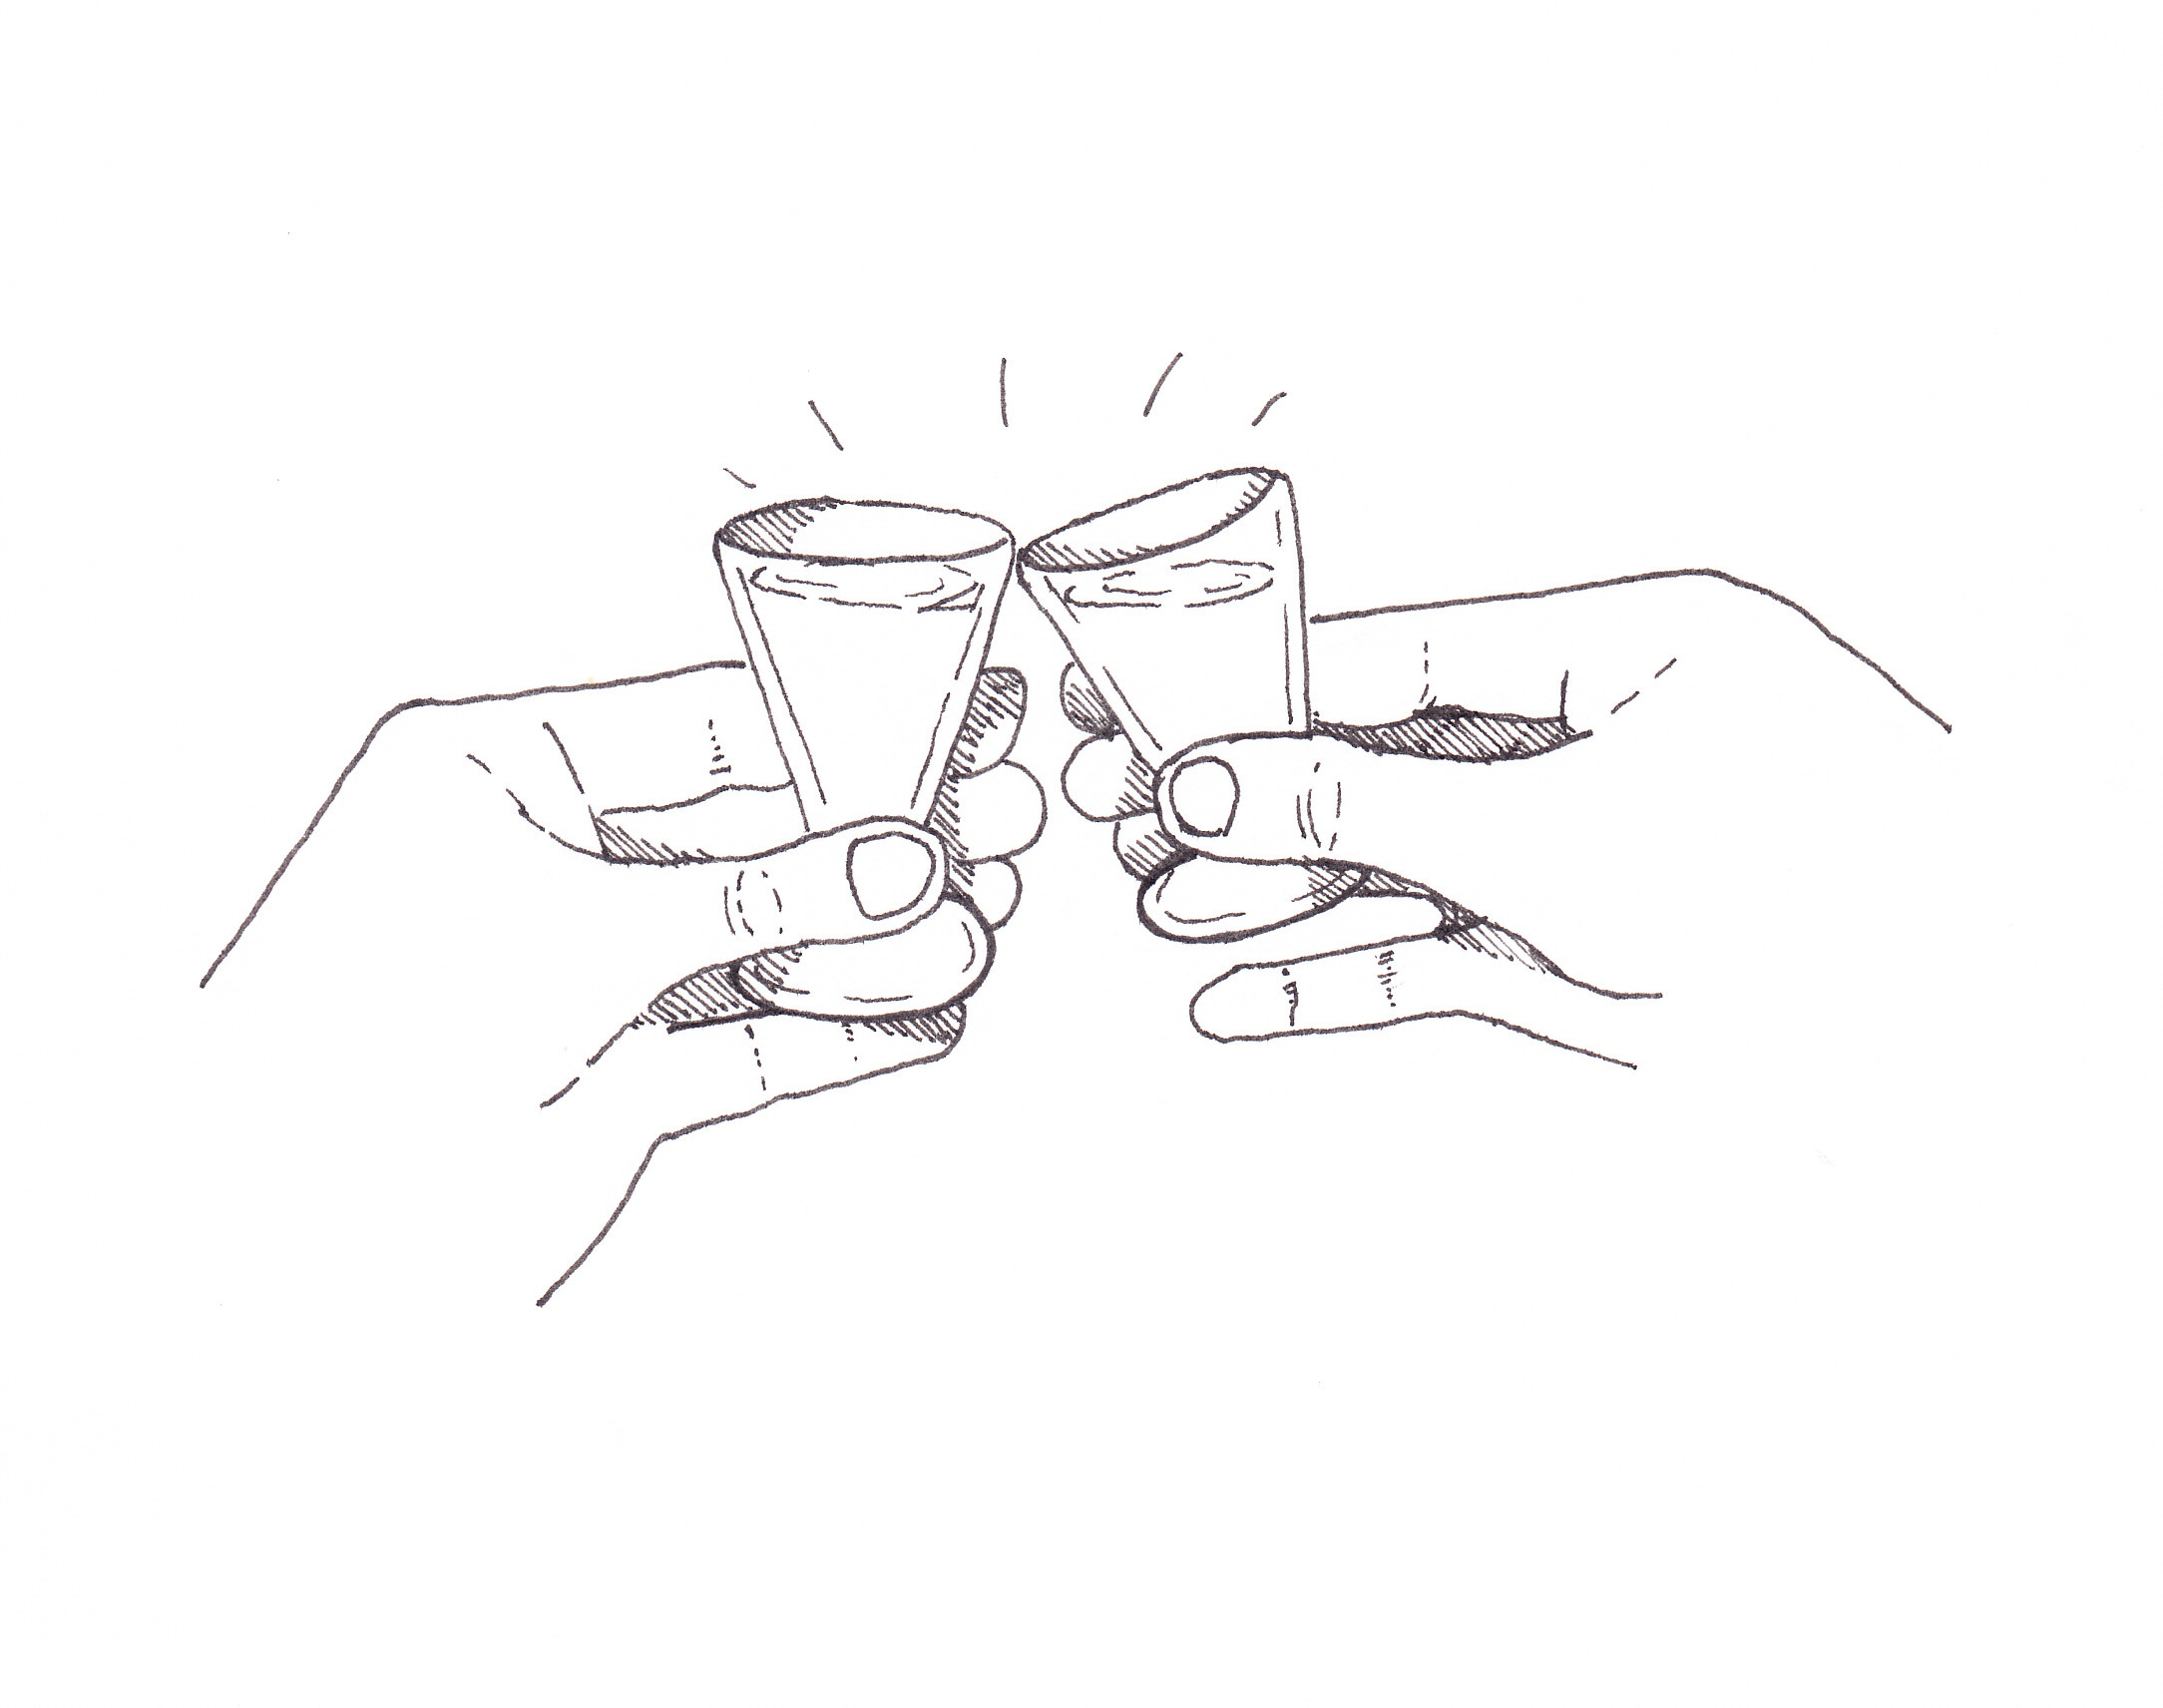
\includegraphics[width=5cm]{../bilder/skalandehander.jpg} 
\end{center}
\end{figure}
\sclearpage
\input{Rullaati.tex}
\sclearpage
\input{Sibbovisan.tex}
\sclearpage
\beginsong{Sörnai gusha}[ 										
	index={Oon vain köyhä poika}]		
	
\beginverse*						
Sörnai gusha nietu Molotova
sörnai gusha herba Moskova.
:,: Njet, njet bonimai votvot risubuska,
dara zeva votvot harasoo. :,:
\endverse

\beginverse				
Isä Stalin ja äiti Hrushtsheva,
iski silmää ginihibragas’.
:,: Oi-oi oisiba vodgaa ollut heillä,
oisi isgu gäynyd alemmas. :,:
\endverse

\beginverse
Siellä missä versoaapi vilja, 
siellä kasvoi kaunis Katjuska.
:,: Katjuskalla koimat on keuhkot,
basga haisee Nevan rannalla. :,:
\endverse

\beginverse
Oon vain köyhä kolhoosinainen,
ei oo mulla yhtään ystävää.
:,: Ei ole lehmää eikä ole lammasta,
eikä suussa yhtään hammasta. :,:
\endverse

\beginverse
Siperian lakeus on suuri,
Sonja siellä lunta lapioi.
:,: Sonjalla kävi hiton huono tuuri,
kun länsituuli uutta lunta toi. :,;
\endverse

\beginverse
Oon vain köyhä poika Petroskoista,
ei oo mulla yhtään ystävää. 
:,: Sirppi ja vasara ne taivahalla loistaa,
basga haisee, balalaikka soi. :,:
\endverse		
\endsong		

\sclearpage
\beginsong{Strunt i sorger}[ 							
	sr={},
	index={Hej dingelidong}]		
	
\beginverse*						
Strunt i sorger och bekymmer,
något roligt skall man ha.
När som livets afton skymmer,
då är det slut på det roliga.
Då går vi ut på vår balkong
och sjunger denna enkla sång:
Hej dingelidong,
HEJ dingelidong,
HEJ dingelidingelidong !
\endverse					

\vspace{5mm}					
\endsong		

\input{TanaanOtetaan.tex}
\sclearpage

\beginsong{Tänk om jag hade lilla nubben}[ 					
	sr={Hej tomtegubbar}]	
	
\beginverse*						
Tänk om jag hade lilla nubben på ett snöre i halsen.
Tänk om jag hade lilla nubben på ett snöre i halsen.
Jag skulle dra den upp och ner,
så att den kändes som många fler.
Tänk om jag hade lilla nubben på ett snöre i halsen.
\endverse						

\vspace{5mm}	
\endsong		
		
\input{TillSpritbolaget.tex}
\sclearpage
\beginsong{Tuborg}		
	
\beginverse*						
:,: Tu tu tu Tuborg 
och ca ca ca Carlsberg 
det är den bästa 
pi pi pi pilsnern som jag vet. :,: 
\endverse						

\beginverse				
:,: Tu tu tu Carlsberg 
och ca ca ca Tuborg 
det är det bästa 
pi pi pi ölet jag vet. :,:
\endverse

\beginverse
:,: Tu ca pi Ölsner och 
pi ta ca bira 
det är den bästa 
ca pi tu lering som jag gjort. :,:
\endverse
\endsong		

\begin{figure}[!b]
\begin{center}
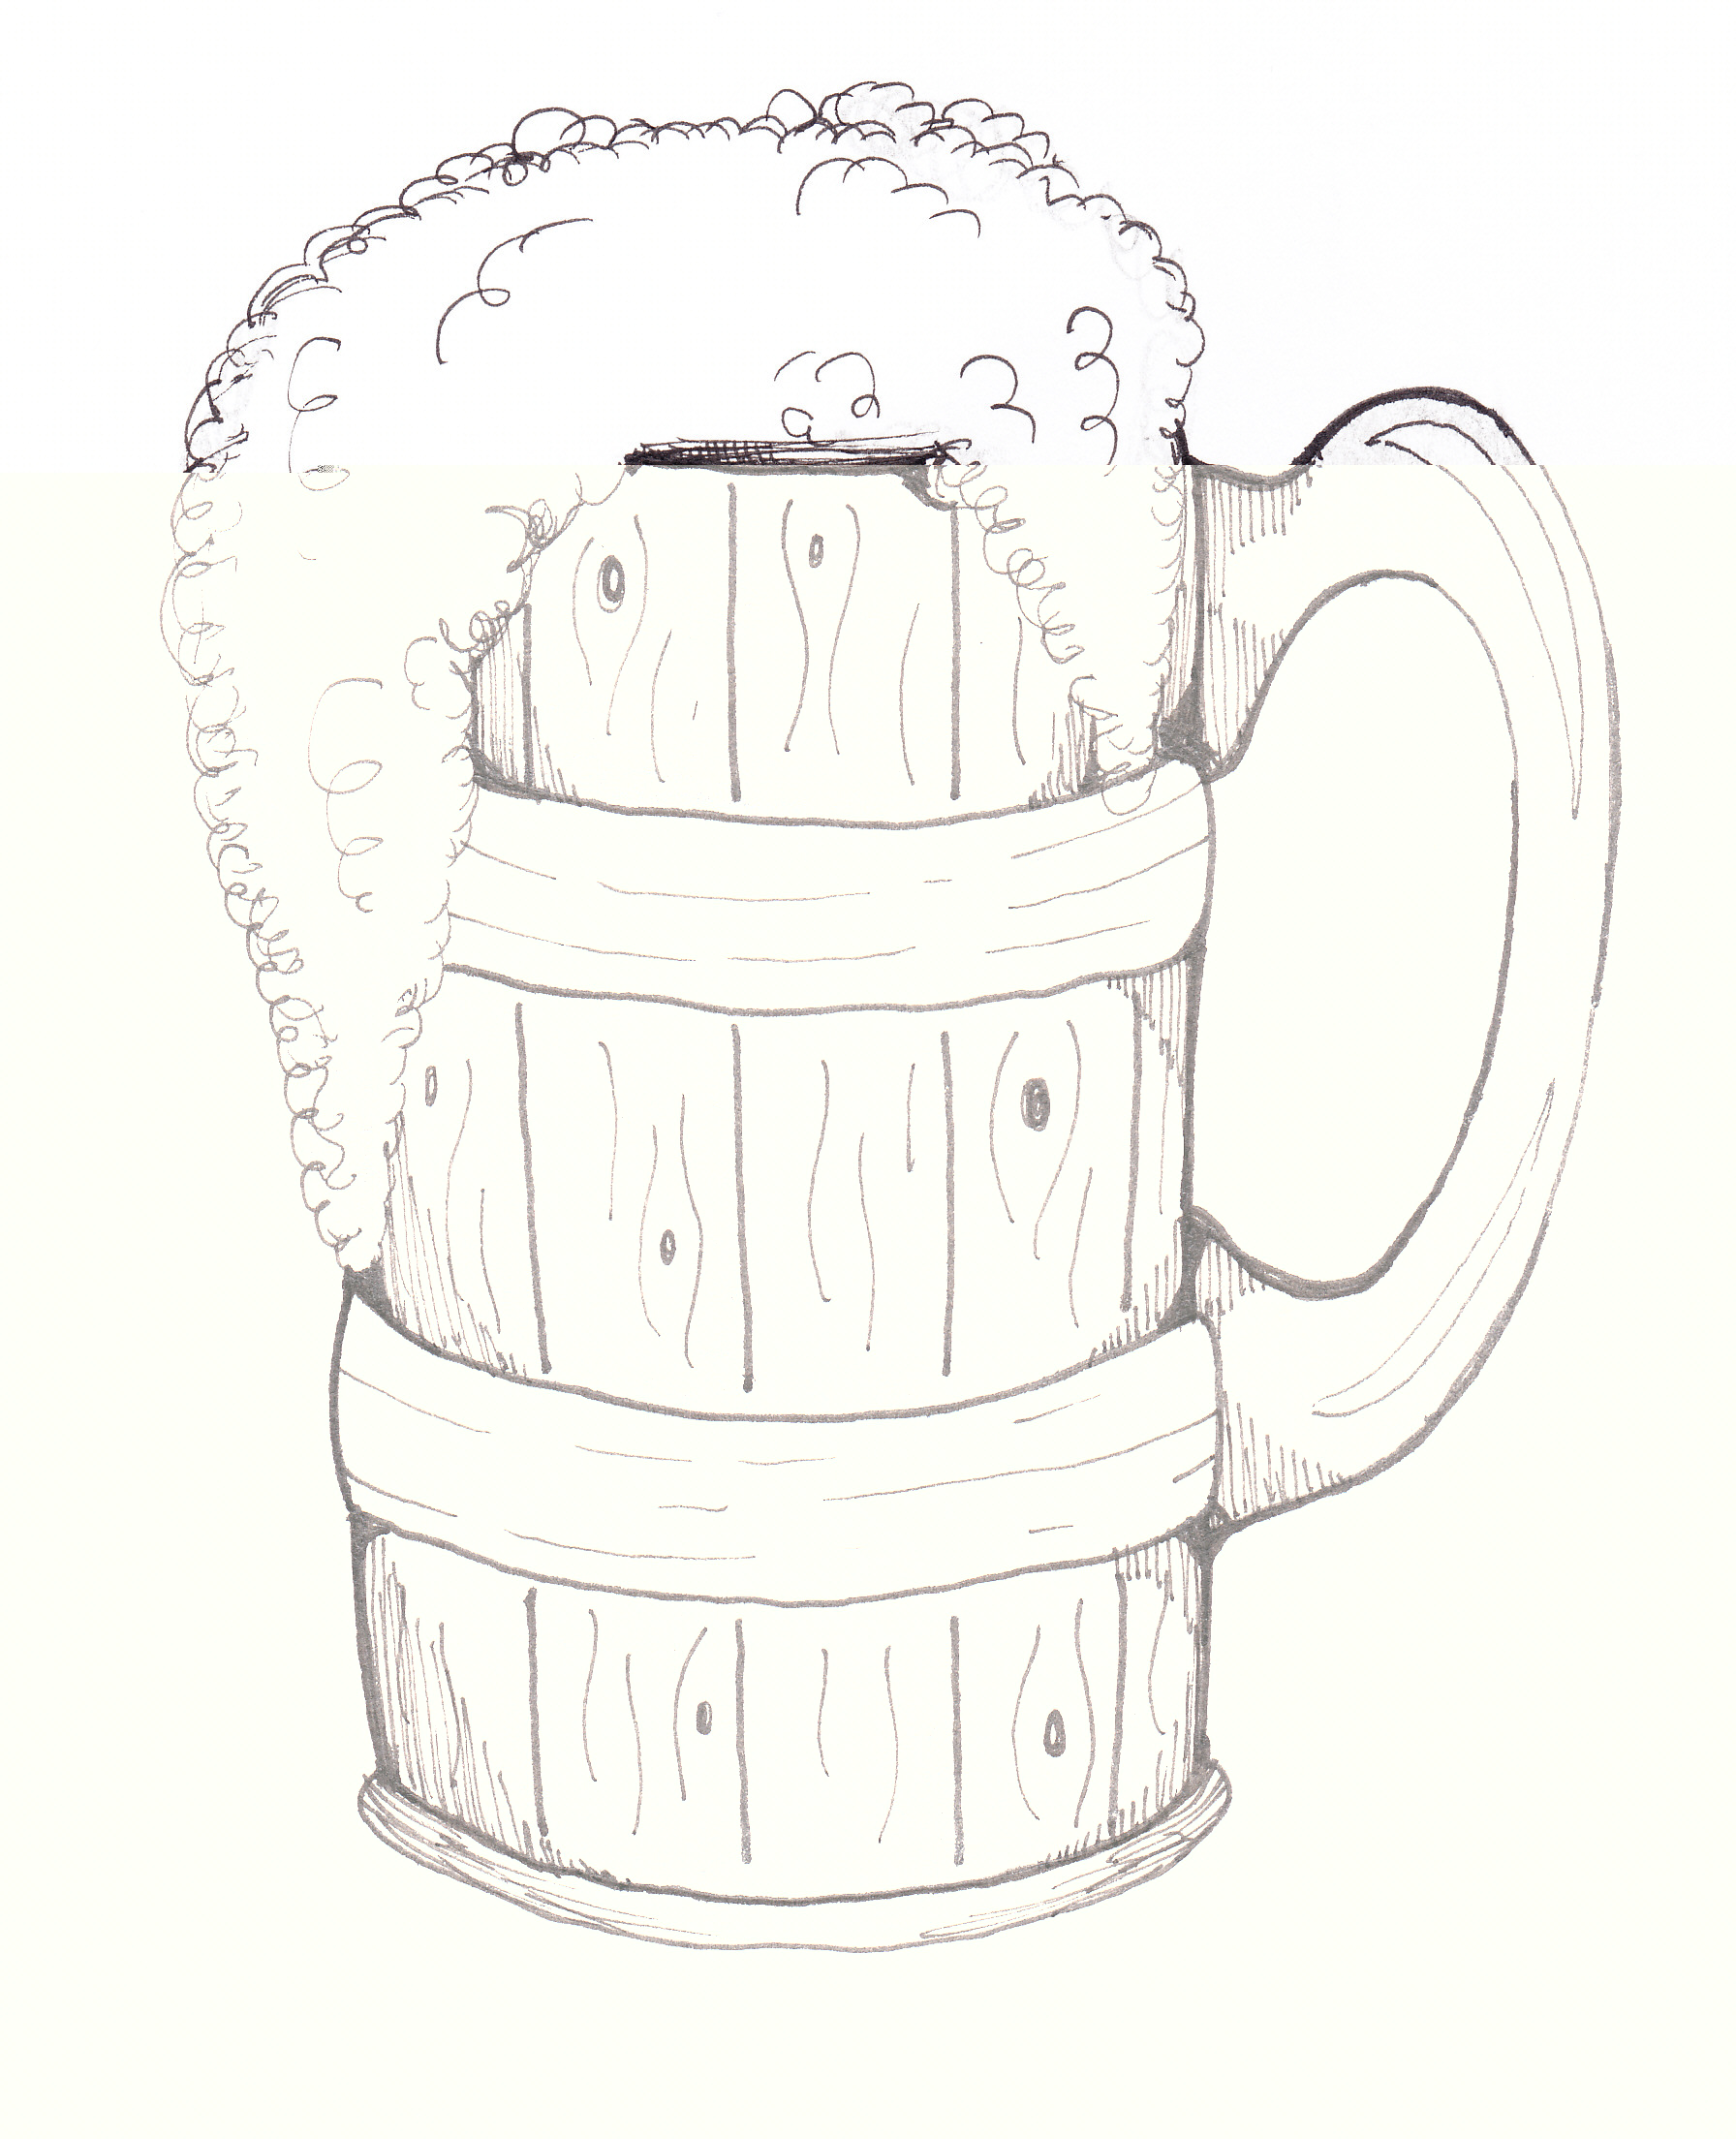
\includegraphics[width=30mm]{../bilder/stop.jpg} 
\end{center}
\end{figure}
\sclearpage
\beginsong{Uti vår mage}[ 							
	sr={Uti vår hage},
	index={Kom Skåne och Aqua Vitae}]		
	
\beginverse*						
Uti vår mage där växa begär,
kom hjärtans kär.
Vill du mig något så träffas vi där. 
Kom Skåne och Aqua Vitae
kom O.P. och allt vad sprit ä'
kom ljuva Genever, kom Överste! 
\endverse				

\vspace{5mm}						
\endsong		

\input{UtiVartBarskap.tex}
\sclearpage
\input{DarSomSadesfalten.tex}
\begin{figure}[!b]
\begin{center}
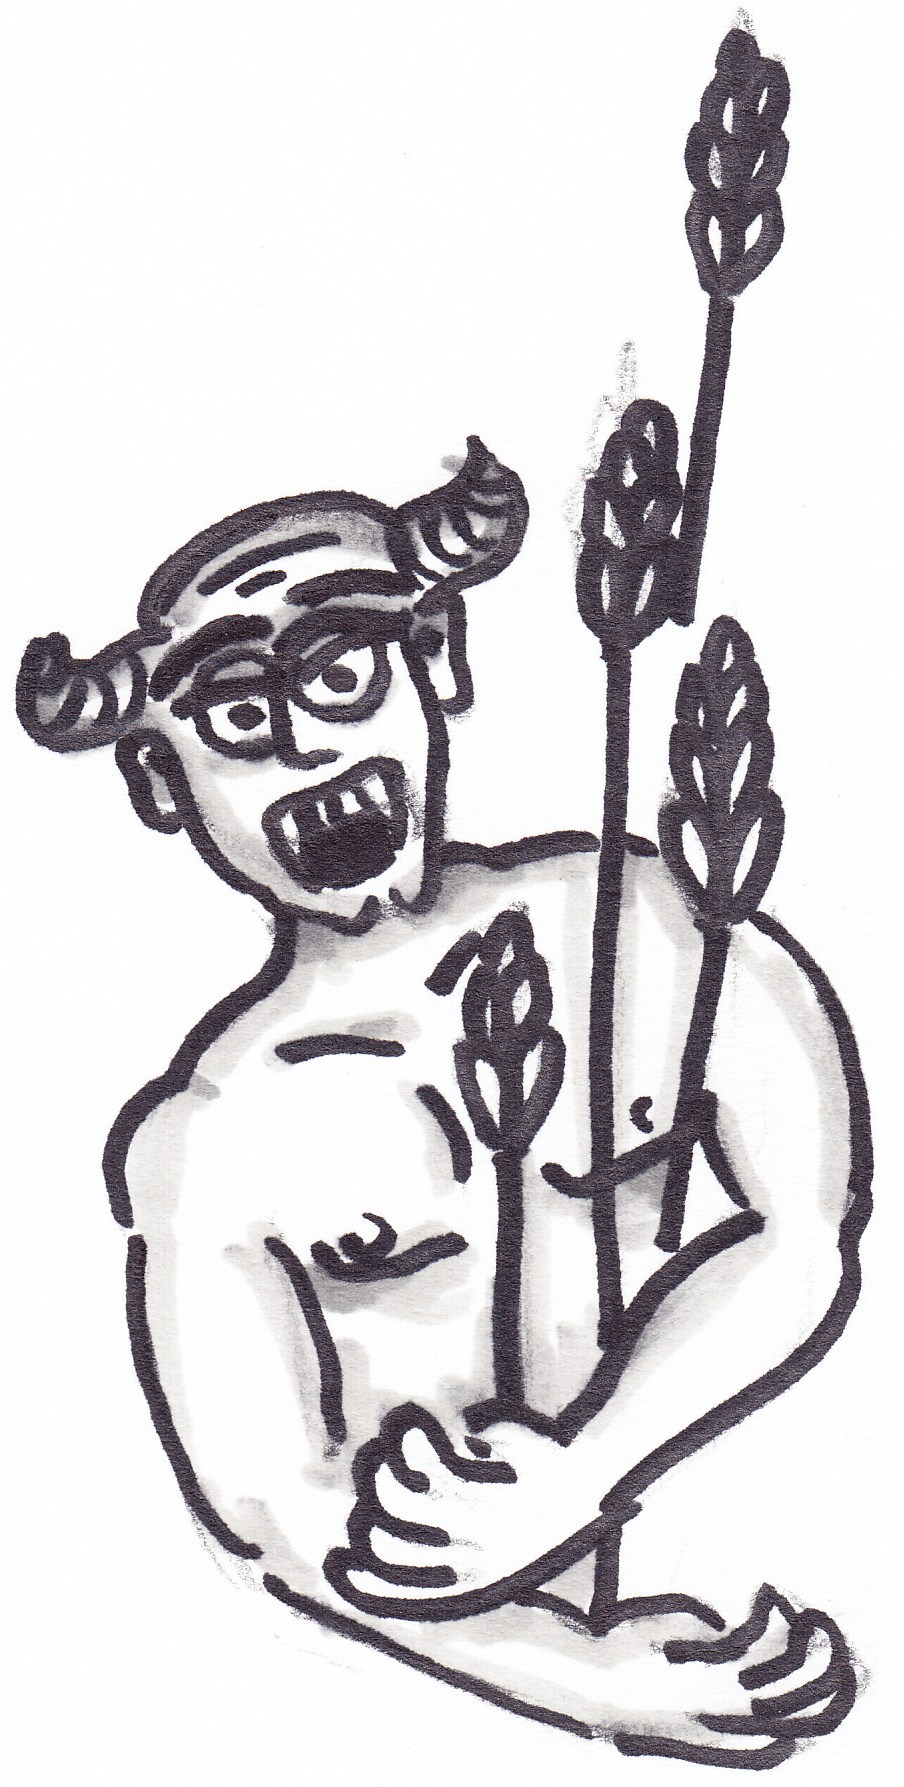
\includegraphics[width=3cm]{../bilder/javel.jpg} 
\end{center}
\end{figure}
\sclearpage
\beginsong{Vem sade ordet}[ 							
	sr={Vårvindar friska}]		
	
\beginverse*						
Vem sade ordet ``skål'' här vid bordet,
viskande for det sällskapet kring.
Fattom kristallen, nubben är kall den,
stiger åt skallen, pling- planga- pling.
Käraste vänner, välkomna hit,
känn hur den doftar god akvavit.
Nu lilla hutten, går i kaputten,
skål lilla tutten, pling- planga- pling.
\endverse		

\vspace{5mm}								
\endsong		

\input{VodkaVodka.tex}
\sclearpage
% Exempel på färdig-formaterad sång till VN:s
% sångbok 2010.

% Denna fil kan användas som sådan, bara verserna,
% namnen och annan rådata behöver bytas ur fälten.
% Tecknet "%" markerar en kommentar som helt och 
% hållet ignoreras av programmet som läser filen.

% Spara den färdiga filen som 
% 'SangnamnUtanMellanslagEllerSkander.tex'
% t.ex. blir "Vid En Källa" till 
% 'VidEnKalla.tex'
% Varje sång blir en egen fil.

\beginsong{Öl, vin, sprit}[ 	% Börja sången här
	by={},	% Författare
	sr={Jenka}			% Melodi
	]		% Alternativa
			% sångnamn
	
\beginverse*		% Börja vers
Öl, vin, sprit och gammal finkel,
har fått mig att se i vinkel.
Därför hamnar inte supen i strupen 
utan i min hörapparat.
Va? Skåååål?
\endverse			% Sluta vers

\vspace{5mm}
\endsong			% Sluta sång

% Exempel på färdig-formaterad sång till VN:s
% sångbok 2010.

% Denna fil kan användas som sådan, bara verserna,
% namnen och annan rådata behöver bytas ur fälten.
% Tecknet "%" markerar en kommentar som helt och 
% hållet ignoreras av programmet som läser filen.

% Spara den färdiga filen som 
% 'SangnamnUtanMellanslagEllerSkander.tex'
% t.ex. blir "Vid En Källa" till 
% 'VidEnKalla.tex'
% Varje sång blir en egen fil.

\beginsong{Jag var full en gång}[ 	% Börja sången här
	by={},	% Författare
	sr={Flottarkärlek}]		% Alternativa
			% sångnamn
	
\beginverse*		% Börja vers
Jag var full en gång för länge sen,
på knäna kröp jag hem,
och på vägen träffa jag en elefant, elefant.
Elefanten börja pinka och jag trodde det var öl,
sedan dess har jag bli'tt kallad
jävla knöl, mera öl!
\endverse			% Sluta vers

\beginverse*		% Börja vers
Jag var full en gång för länge sen,
på knäna kröp jag hem,
varje dike var för mig ett vilohem, vilohem.
I varje hörn och varje vrå så hade jag en liten vän,
ifrån renat upp till 96 procent, mera sprit!
\endverse			% Sluta vers

\beginverse*		% Börja vers
Haderian haderej haderian hadera
Utan sprit går det inte bra
Haderian haderej haderian hadera
Lilla snapsen nu vi ta!
\endverse			% Sluta vers
\endsong			% Sluta sång

\sclearpage
\beginsong{Vikingen}[
		sr={When Johnnie Comes Marching Home},
		index={En viking vill ha livets vann}]

\beginverse
En viking vill ha livets vann
Hurra, hurra!
Den hastigt i mitt svalg försvann
Hurra, hurra!
Till kalv, till oxe, till fisk, till fläsk
När kärringen bara dricker läsk
Då vill alla vikingar ha en besk. 
\endverse

\beginverse
När vi har druckit besken slut
Tragik, tragik!
Då bäres varje viking ut
som lik, som lik
och sen om vi vaknar vi sjunger en bit,
så korkar vi upp Skånes akvavit.
Skål för alla vikingar som kom hit!
\endverse
\endsong
\sclearpage